\section{Aufbau und Durchführung}
\subsection{Aufbau}
\label{sec:Aufbau}
Im vorliegenden Versuchsaufbau wird ein kleiner Wagen mit Rollen betrachtet, welcher sich auf einer Schiene befindet.
Mithilfe eines befestigeten Seils, verbunden mit einem Synchronmotor, kann dieser Wagen auf der Strecke in zehn verschiedenen wählbaren konstanten Geschwindigkeitseinstellungen vorwärts oder rückwärts zurücklegen.
Auf dem Wagen kann ein Lautsprecher befestigt werden, welcher Töne wiedergeben kann.
Diese werden mithilfe einer frequenzstabilen Generators erzeugt.\\
Am Ende der Strecke befindet sich ein Mikrophon, welches eine Signalspannung erzeugt die im Folgenden zur Betrachtung der aufgenommenen Wellen verwendet werden kann.\\
Zudem sind zwei Lichtschranken vorhanden, die an der Schiene montiert werden können und somit das Durchfahren des Wagens registrieren können.
Sie funktionieren, indem eine Infrarot-Lichtquelle einen konstanten Lichtstrahl auf einen gegenüberliegenden Phototransistor sendet.
Sobald die Verbindungsstrecke zwischen beiden Elementen unterbrochen wird, bricht der Strom im Transistor zusammen.
Dieser Impuls kann ebenfalls im weiteren verwendet werden.\\
Um die genannten Impulse verarbeiten zu können, sind mehrere Bauteile mit logischen Funktionen vorhanden.
Diese können die Impulse des Mikrophons sowie der Lichtschranke jedoch nur als TTL-Signale verarbeiten, so dass diese zunächst durch einen Schmitt-Trigger umgewandelt werden müssen.

\subsection{Durchführung}
\subsubsection{Bestimmung der Wagengeschwindigkeiten}
Die zehn verschidenen Wagengeschwindigkeiten können, da es sich um lineare Bewegungen handelt, mit dem Weg-Zeit-Gesetz bestimmt werden.
Der Aufbau ist in Abbildung \ref{tfig:1} dargestellt.
\begin{figure}
  \centering
  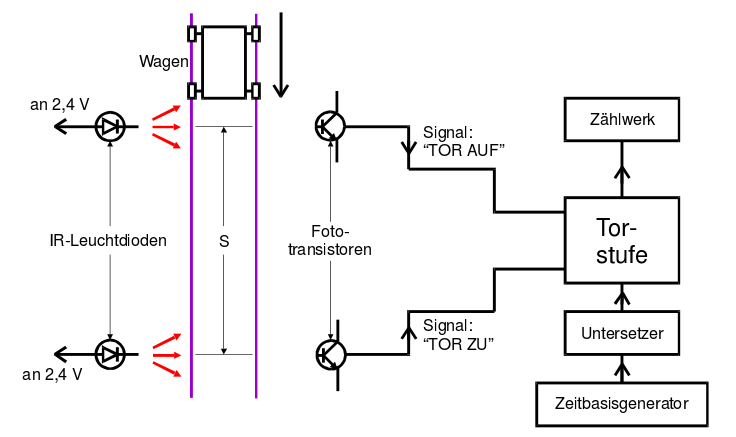
\includegraphics[height=5cm]{aufbau1.png}
  \caption{Aufbau zur Bestimmung der Wagengeschwindigkeiten.}
  \label{tfig:1}
\end{figure}
Mithilfe eines Maßbandes wird die Strecke zwischen zwei an der Strecke montierten Lichtschranken gemessen.
Ein Zeitbasisgenerator liefert nun konstante Impuls im zeitlichen Abstand von $\SI{1}{\micro\second}$.
Mithilfe eines dekadischen Untersetzes wird das Signal nun so verändert, dass die Häufigkeit der Impulse dem zeitlichen Rahmen des Experimentes angepasst wird.
Hier sollen nur alle $\num{e-4}$ zeitliche Impulse abgegeben werden. \\
Sobald der Wagen die erste Lichtschranke passiert, wird dieser Impuls von einer bistabilen Kippstufe registriert.
Dieser speichert diesen Impuls und behält ihn solange, bis durch die zweite Lichtschranke ein weiterer Impuls abgegeben wird.
Der gespeicherte Impuls äußert sich in einem anliegenden Potential.
Dieses Potential wird mit einem UND-Gatter mit dem Zeitsignal des dekadischen Untersetzers verbunden und an ein Zählwerk weitergegeben.
Dementsprechend misst das Zählwerk die Impulse und somit die Zeit die vergeht, während der Wagen sich zwischen den beiden Lichtschranken befindet.\\
Die agegebene Messung wird für alle zehn Geschwindigkeiten jeweils fünf mal wiederholt.

\subsubsection{Frequenzmessung}
Um die Frequenzverschiebung zwischen einem bewegten Sender sowie einen festen Empfänger zu bestimmen, wird der Lautsprecher auf dem Wagen montiert.
Es soll die Anzahl der Schwingungen, die der Empfänger in einem fest eingestellten Zeitraum registriert, bestimmt werden.
Der Versuchsaufbau ist in Abbildung \ref{tfig:2} dargestellt.
\begin{figure}
  \centering
  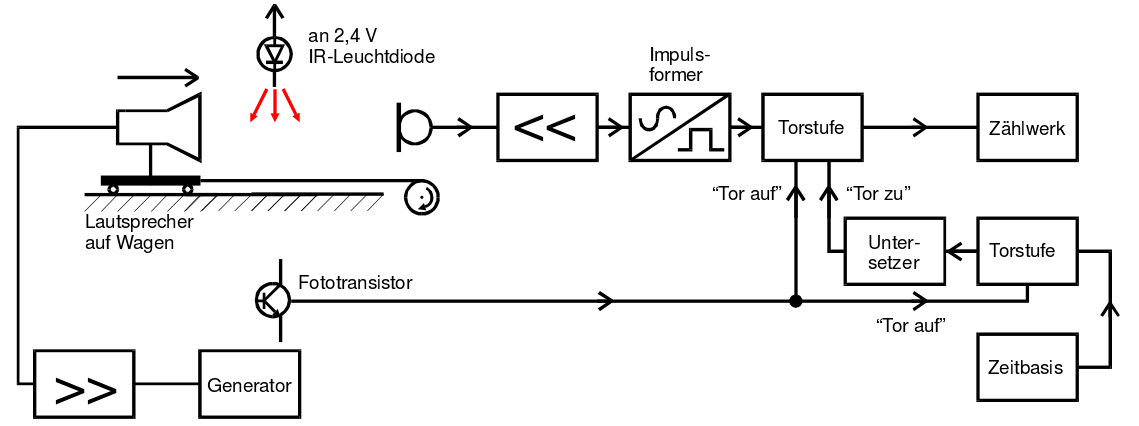
\includegraphics[height=5cm]{aufbau2.png}
  \caption{Aufbau zur Bestimmung der Frequenz des Empfängers.}
  \label{tfig:2}
\end{figure}
Es wird eine Lichtschranke benötigt, welche den Start der Messreihe darstellt.
Sobald diese vom Wagen passiert wird, speichert die bistabile Kippstufe den Impuls.
Mithilfe eines UND-Gatters werden, zusammen mit dem Zeitbasisgenerator, Zeitsignale an den Untersetzer geliefert.
Dieser zählt die eingehenden Zeitimpulse und gibt solange ein Signal aus, bis der voreingesteller Untersetzungsfaktor erreicht ist.
Mit ihm kann somit widerum das Zeitintervall der Messung eingestellt werden.
Das konstante Signal des Untersetzers wird mit dem Signal der bistabilen Kippstufe an ein UND-Gatter angelegt und an das Zählwerk weitergegeben.
Somit ist gewährleistet, dass nur während eines durch den Untersetzer festgelegten Zeitraumes die Schwingungen die der Empfänger erhält, gezählt werden.
Aus der Kenntnis der Schwingungen pro Zeiteinheit kann nun die Frequenz bestimmt werden.\\
Dieses Messverfahren wird für alle Geschwindigkeiten jeweils fünf mal für den sich vom Mikrophon entfernenden Sender sowie jeweils fünf mal für den sich zum Mikrophon zubewegenden Sender durchgeführt.
Zusätzlich werden Messungen bei einem stehenden Wagen durchgeführt, um die Ruhefrequenz zu erhalten.
